\documentclass[tikz]{standalone}
\usepackage{pgfplots}
\pgfplotsset{compat=1.15}
\usepackage{mathrsfs}
\usetikzlibrary{arrows,calc}
\usepackage{tkz-euclide}
\pagestyle{empty}

\definecolor{AngleClr}{rgb}{0,0.39215686274509803,0}
\definecolor{ShapeClr}{rgb}{0.6,0.2,0}

\begin{document}

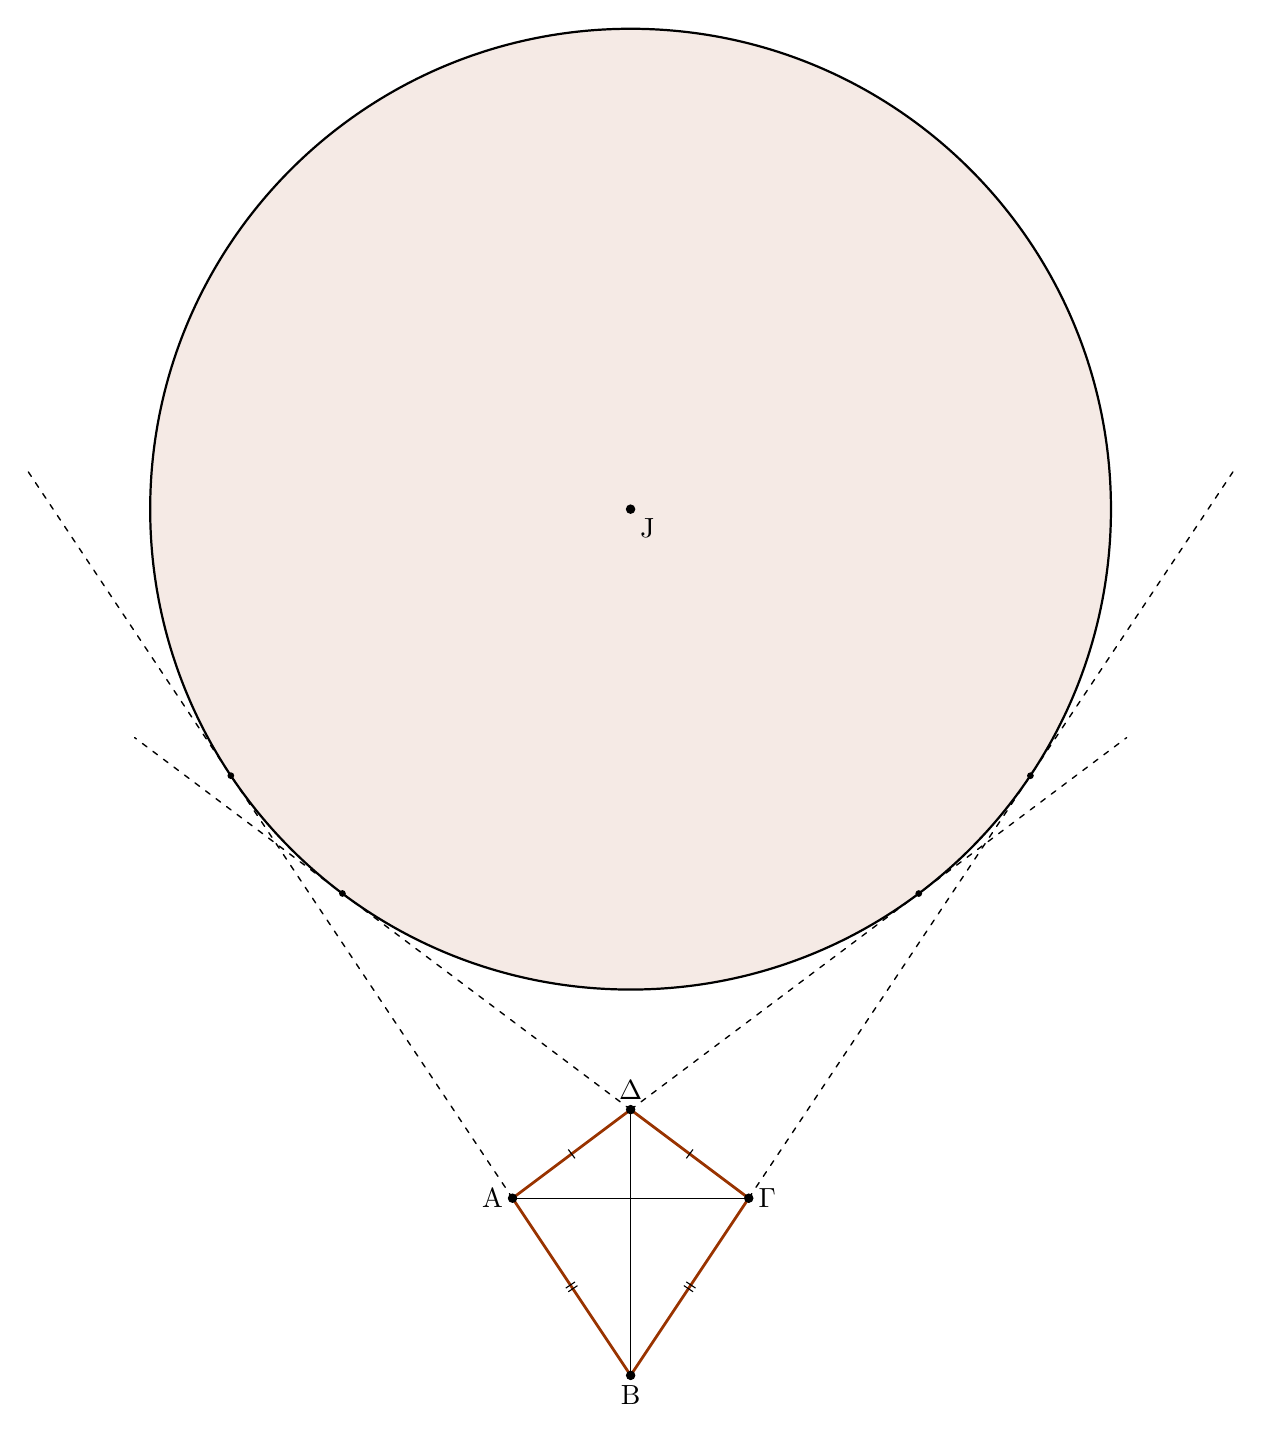
\begin{tikzpicture}[scale=.75]
\tkzSetUpLine[line width=1pt,color=black]
\tkzSetUpPoint[fill=black]

\tkzDefPoints{0/0/A,4/0/C,2/1.5/D,2/-3/B}

\tkzFillPolygon[fill=white](A,B,C,D)


\tkzInterLL(C,D)(B,A) \tkzGetPoint{BAA}
\tkzInterLL(A,D)(B,C) \tkzGetPoint{BCC}
\tkzDefPointOnLine[pos=1.7](B,BAA)\tkzGetPoint{AA}
\tkzDefPointOnLine[pos=1.7](B,BCC)\tkzGetPoint{CC}

\tkzDrawSegments[line width=0.5pt,color=black,dashed,dash pattern=on 2pt off 2.75pt](A,AA C,CC)


\tkzDefLine[bisector](C,BAA,AA)\tkzGetPoint{a}
\tkzDefLine[bisector](A,BCC,CC)\tkzGetPoint{b}
\tkzInterLL(BAA,a)(BCC,b) \tkzGetPoint{I}
\tkzDefPointBy[projection=onto A--B](I) \tkzGetPoint{Ia}
\tkzDefPointBy[projection=onto B--C](I) \tkzGetPoint{Ib}
\tkzDefPointBy[projection=onto C--D](I) \tkzGetPoint{Ic}
\tkzDefPointBy[projection=onto D--A](I) \tkzGetPoint{Id}

\tkzDrawCircle[black,fill=ShapeClr,fill opacity=0.1,line width=0.8pt](I,Ia)

\tkzDrawSegments[line width=0.5pt,color=black](A,C B,D)
\tkzDrawSegments[line width=0.5pt,color=black,dashed,dash pattern=on 2pt off 2.75pt, add=0 and 0.4](D,BAA D,BCC)

\tkzDrawPolygon[color=ShapeClr](A,B,C,D)
\tkzDrawPoints[size=3](A,B,C,D,I)
\tkzDrawPoints[size=2](Ia,Ib,Ic,Id)
\tkzLabelPoint[left](A){$\rm A$}
\tkzLabelPoint[below](B){$\rm B$}
\tkzLabelPoint[right](C){$\rm \Gamma$}
\tkzLabelPoint[above](D){$\rm \Delta$}
\tkzLabelPoint[below right](I){$\rm J$}

\tkzMarkSegments[mark=|,size=2](D,A D,C)
\tkzMarkSegments[mark=||,size=2](B,A B,C)

\end{tikzpicture}

\end{document}
